\chapter{序論}
\thispagestyle{empty}
\label{Chap1}
\minitoc

\newpage
%%%%%%%%%%%%%%%%%%%%%%%%%%%%%%%%%%%%%%%%%%%%%%%%%%%%%%%%%%%%%%%%%%%%%%%%%%%%%%%

%==============================================================================
%背景
%==============================================================================
\section{背景}
\label{Background}
建設業は,道路、河川などの社会資本や産業施設,公共施設の整備・維持管理を行い,国内総生産及び就業者数の約10%を占める基幹産業の一つである.\cite{日本建設組合連合2016}
\par 2010 年に発生した東日本大震災や各地の豪雨災害時での復興活動などで,建設業の重要性が再認識されている.
しかし,近年の建設業界では,技能労働者の高齢化や就業者の減少により熟練オペレーター不足が問題となってい
る.また,国土交通省の「建築産業の現状と課題」\cite{建設経済研究所2017}によると,2015 年の技能労働者数は330 万人であり,10 年後
の 2025 年は 286 万人と減少すると試算されている.今後,深刻な人材不足の危機に陥ると予想されており,人材不
足を補う為,建設現場における作業の自動化は重要な課題である.
\par
現場における作業で自動化の要求の高い作業の一つが,バックホウとダンプトラックの連携による土砂積み込み作業の自動化である.
土砂の積み込みの際には,ダンプトラックは運転手により積み込み可能な位置まで移動されるが,バックホウによる積み込み作業を自動化するために
は,バックホウに対するダンプトラックの相対的な位置姿勢を正しく獲得する必要がある.
一般の作業現場では,GNSSやTotal Stationによって位置姿勢の把握\cite{土井下2010}が行われているが,GNSS等の衛星測位システムで高精度な位置姿勢を獲得するためには,通信基地局などの環境整備が必要であり,設備コストが大きいことが課題である.
Tostal Stationは建機に搭載されたプリズムにレーザーを照射することで高精度な位置情報を獲得できるが,一旦,レーザー照射が途切れるとプリズムを
追従できない問題がある.
そのため,環境に大がかりな設備を要さずに位置姿勢を計測する手法が期待されている.
%%%%%
\begin{figure}[b]
 \begin{center}
 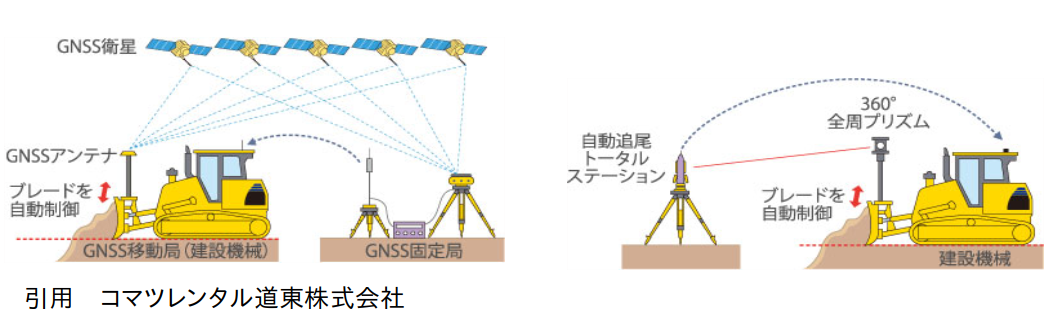
\includegraphics[width=1.0\columnwidth]{./chap1/fig/GNSS.png}
 \caption{GNSSやTSによる位置情報の把握}
 \label{fig:GNSS}
 \end{center}
 %\vspace{-5mm}
\end{figure}
%%%%%

\newpage

\section{従来研究}
対象物体にセンサを搭載せずに外部からのセンシングによる位置姿勢推定の手法が研究されており,マニピュレータによるピッキング作業のための物体検出や
自動運転ための車両の検出などを目的とした研究が多くされている.

ピッキング作業ための物体検出として,RGB-Dセンサの計測結果と対象物体のCADモデルとの照合による3次元物体計測が検討されてきた.\cite{中原智治2001}\cite{林2008}\cite{西卓郎2014}
また近年では深層学習を取り入れたアプローチも増えており,対象物体のあらゆる姿勢の画像をCADデータから生成したものを教師データとした深層学習による推定手法\cite{Sundermeyer2018}\cite{Tremblay2018}などがある.
しかし,実際の作業現場では様々なメーカーのダンプトラックが行き交い,また荷台部も現場によって異なるため,事前にCADデータを用意するのは難しい.

また,車両を対象とした位置姿勢推定の手法としてLIDARを用いた3次元物体検出がある.\cite{Zhang2017}\cite{Chen2017}\cite{Lang2019}\\
図のように広域にレーザーを照射することにより計測した3次元点群から対象物体の点群を検出することで位置姿勢推定を行う.
しかし,土砂積み込み作業は高低差がある環境が多く,LIDARは視野角が狭いため近距離が死角になる.また,LIDARを傾けることで死角を
減らせるが,距離によっては対象物体にレーザー当たらず計測ができない状況が生じる.

\newpage
\section{研究の目的}
1.1 節で述べたように,環境に大がかりな設備を要せずにダンプトラックの位置姿勢を計測する手法が求められている.
そのため,Cバックホウに搭載したRGB-Dセンサから得られるダンプトラックの3次元データを用いた点群位置合わせに基づく位置姿勢推定が有効だと考えられる.
しかし,RGB-Dセンサは点群位置合わせを行う上で有効な高密度の3次元点群を得られるが,計測距離が短く計測できる範囲は狭く,
実際の土砂積み込み作業の際は,ダンプトラックは遠方からバックホウに向かって進入してくる場合が多く,ダンプトラックの進入を判断するためには,
遠方にあるダンプトラックの存在とその大まかな位置姿勢を計測する必要がある.



\par
そこで,本研究では
    \begin{screen}
        \begin{center}
        計測範囲の拡張と距離センサの計測範囲外でも計測可能なダンプトラックの位置姿勢推定手法の提案
        \end{center}
    \end{screen}
を目的とする
\newpage
\section{本論文の構成}
本論文は全4章から構成されている.図に本論文の構成を示す.\par
第1章では,本研究の背景,従来研究,目的について述べた.\par
第2章では,画像認識と点群位置合わせによるダンプトラックの位置姿勢推定の提案手法について述べる.\par
第3章では,本提案手法の有効性を検証するために行った実験について述べる.\par
第4章では,結論と今後の展望を述べる.
\begin{figure}[b]
    \begin{center}
    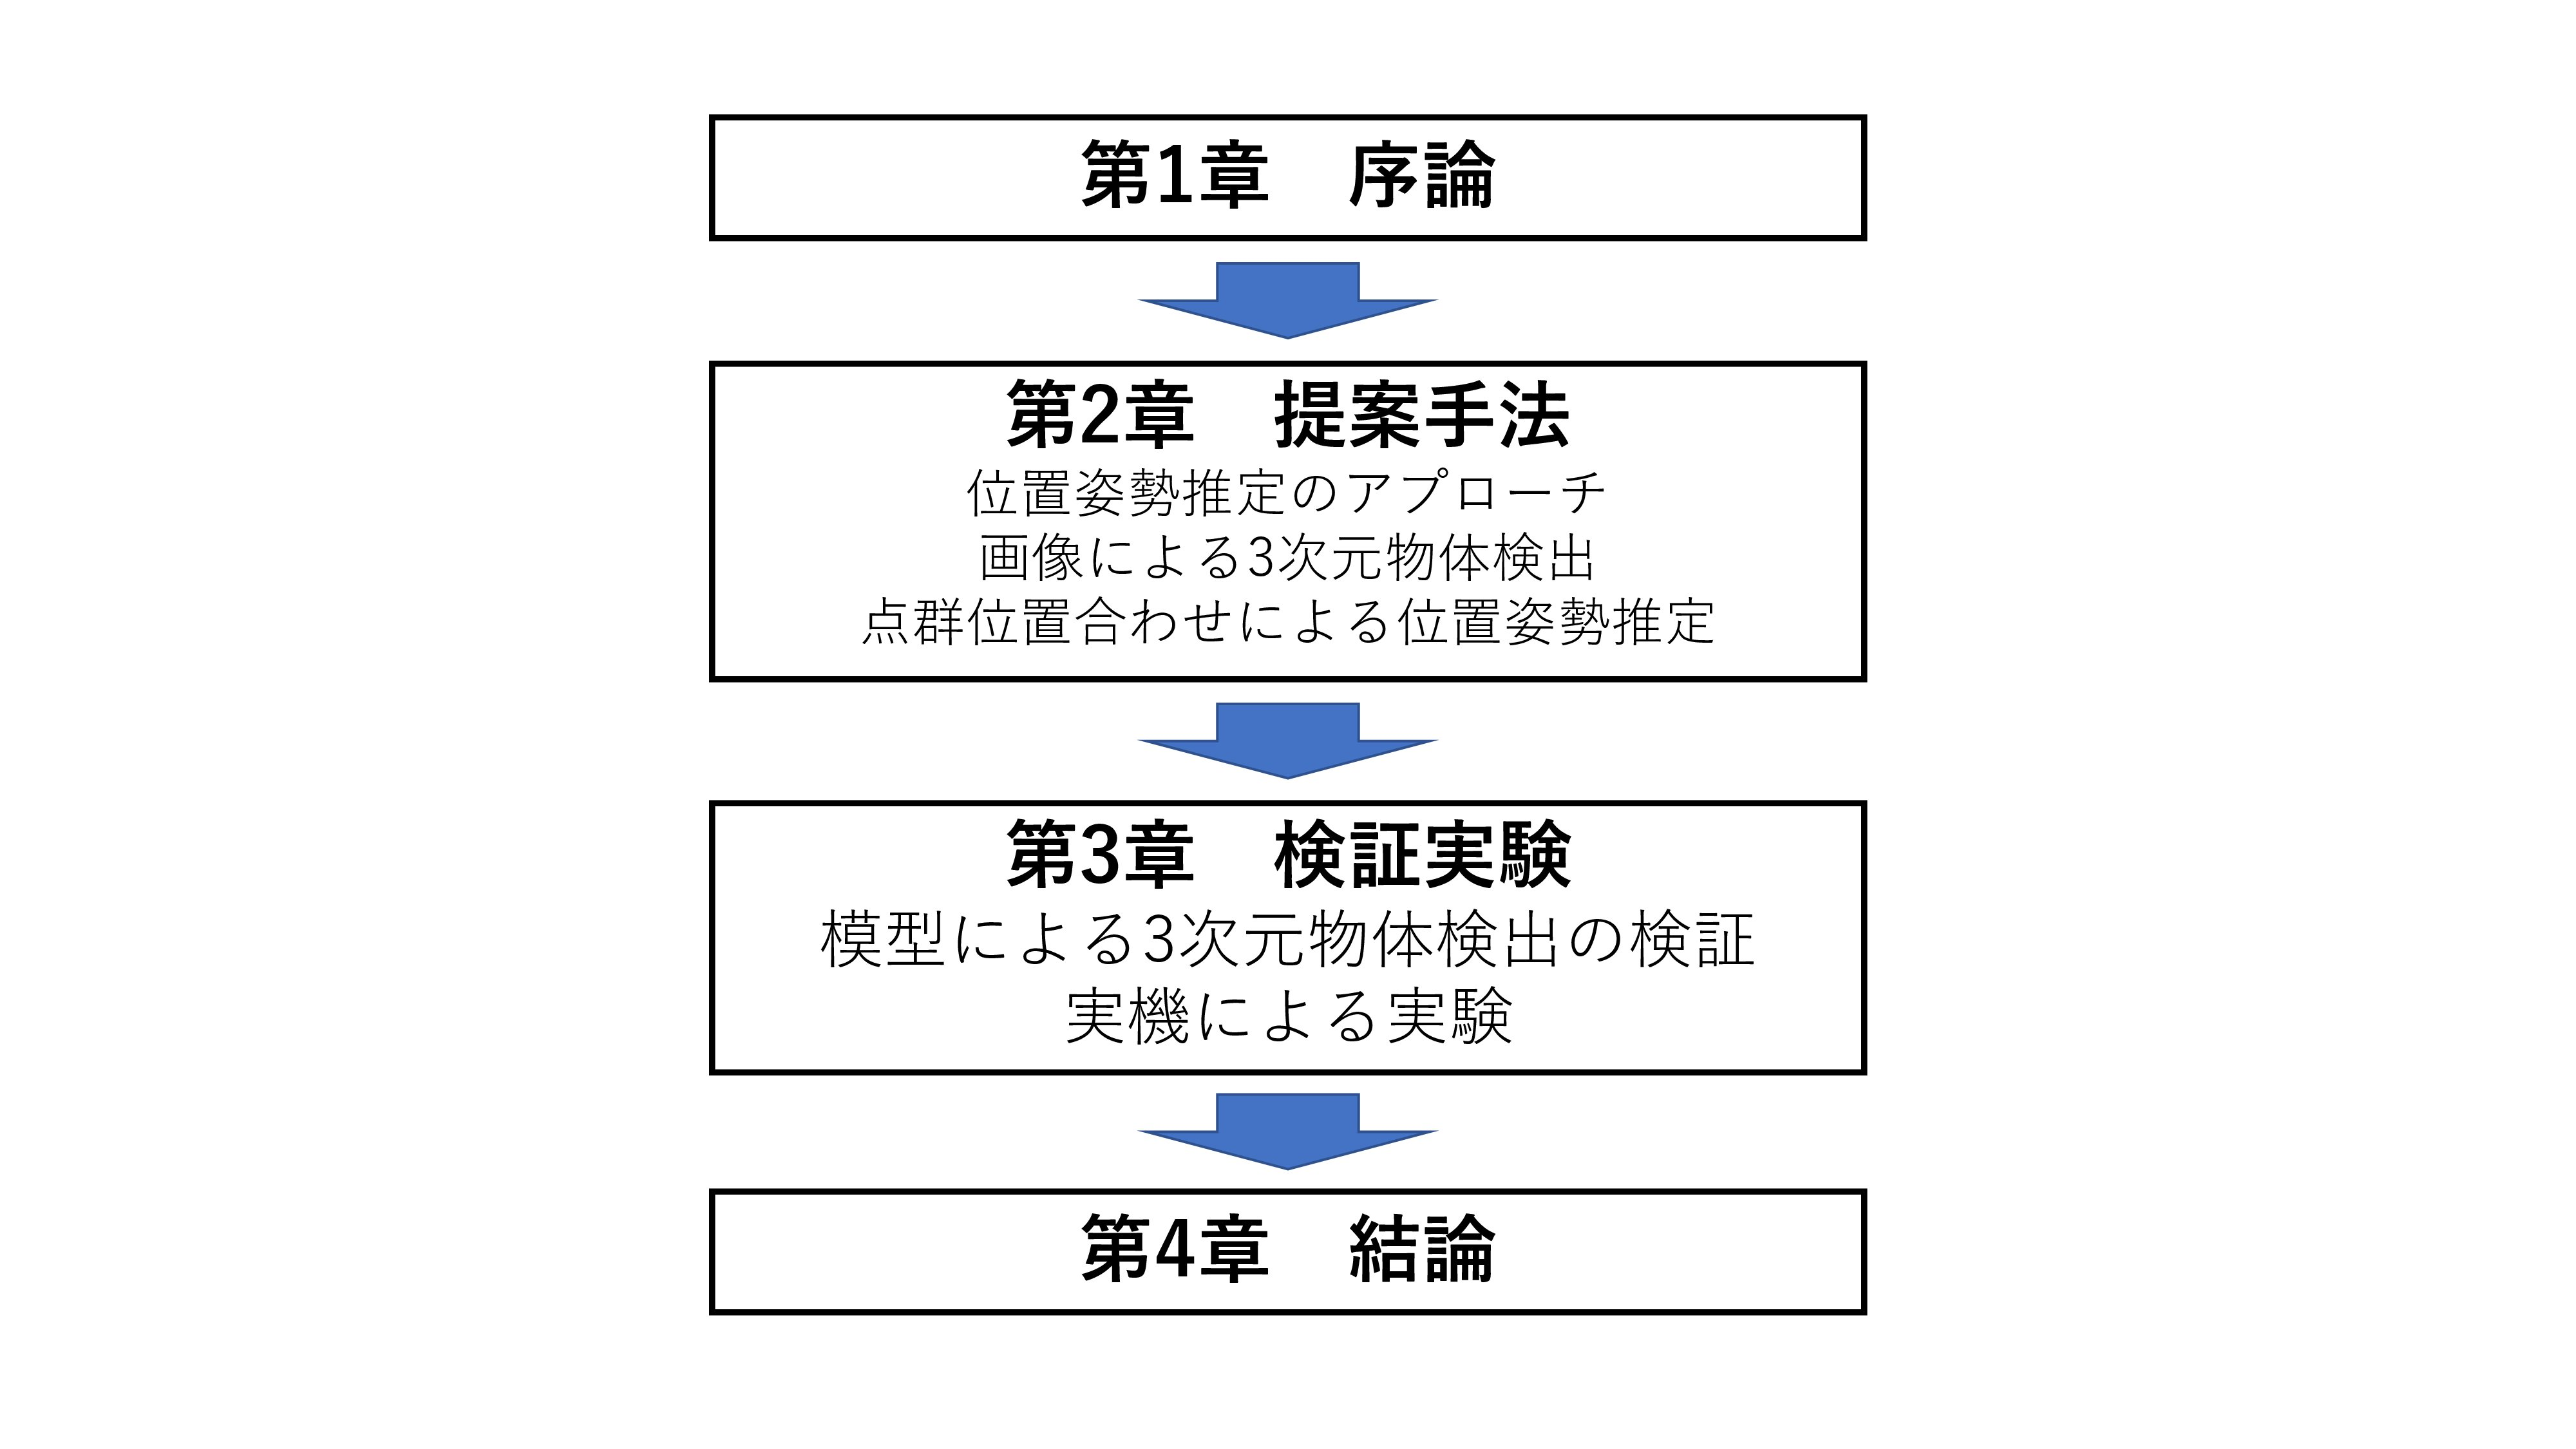
\includegraphics[width=0.3 \columnwidth]{./chap1/fig/struct.jpg}
    \caption{本論文の構成}
    \label{fig:flow}
    \end{center}
    %\vspace{-5mm}
   \end{figure}

%%%%%%%%%%%%%%%%%%%%%%%%%%%%%%%%%%%%%%%%%%%%%%%%%%%%%%%%%%%%%%%%%%%%%%%%%%%%%%%
%%% Local Variables:
%%% mode: katex
%%% TeX-master: "../thesis"
%%% End: